\documentclass[11pt]{article}
\usepackage[margin=1in]{geometry}
\usepackage{booktabs}
\usepackage{hyperref}
\usepackage{times}
\usepackage{amsmath}
\usepackage{amssymb}
\usepackage{tikz}

\title{AgentGuard: Deterministic Security Linting\\for AI Agent Definitions}
\author{Ying Chen}
\date{\href{https://doi.org/10.5281/zenodo.21420490}{doi:10.5281/zenodo.21420490}}

\begin{document}
\maketitle

\begin{abstract}
AI coding harnesses execute agents defined in plain markdown-with-frontmatter files: a tool grant,
a description, and natural-language instructions. These definitions are security-relevant code---a
definition that reads untrusted content while holding shell or network tools is one injected
sentence away from remote code execution or data exfiltration---yet they ship without any static
analysis. We introduce AgentGuard, a deterministic, zero-dependency security linter for agent,
command, and skill definitions. AgentGuard parses each definition's capability grant, models
untrusted-input sources and dangerous sinks, and reports severity-ranked findings for capability
chains such as injection-to-execution, exfiltration paths, and disabled human-in-the-loop
guardrails, each mapped to OWASP LLM Top-10 and MITRE ATLAS. On a gated benchmark of 15 vulnerable
and 13 safe definitions, AgentGuard achieves 0.93 recall and 1.00 precision with zero false
alarms---where naive grant-based or keyword-grep flagging reaches at most 0.47 recall at 0.58
precision---and its security decisions are stable across 81 metamorphic adversarial rewrites; the
single missed case is a named, documented recall boundary rather than a silent gap. Field studies
of the official Claude Code plugin marketplace at two snapshots one month apart (33 and 84 unique
definitions) found 85--86\% lacked any injection guard and 37--39\% could be driven to run a
command or write a file by content they read---rates that held as the marketplace grew
$2.5\times$ and replicated on an independent third-party corpus (95\% unguarded, 50\% chain).
Scanning is cheap: the full marketplace lints in under a second ($\approx$9\,ms per definition). The core claim is narrow: privilege risk in agent definitions can be a deterministic,
benchmark-gated CI check rather than a manual review afterthought.
\end{abstract}

\section{Introduction}
Indirect prompt injection is a structural property of LLM agents, not an implementation bug: any
agent that reads attacker-influenced content and holds action-capable tools can be redirected by
instructions embedded in that content \cite{greshake2023indirect,perez2022ignore,willison2022prompt}.
Modern coding harnesses make this concrete at scale. An agent definition is a markdown file with
YAML frontmatter declaring a name, a description, and a \texttt{tools:} grant; the body is a
natural-language system prompt. A definition that says ``summarize the file'' while granting
\texttt{Bash} is an unguarded injection-to-execution chain---the file being summarized can carry
the instruction \texttt{curl \ldots | sh}, and nothing in the definition tells the model to treat
read content as data.

These files are code. They are committed to repositories, distributed through plugin marketplaces,
installed onto developer machines, and executed with filesystem, shell, and network access. Yet
unlike the application code they sit beside---linted by Bandit, Semgrep, and a CI wall of static
analysis \cite{bandit2024,semgrep2024}---agent definitions ship with no static check at all.
Guidance exists as taxonomy (OWASP LLM Top-10, MITRE ATLAS \cite{owasp2025llm,mitre2024atlas}) and
as design advice \cite{anthropic2024agents}, but not as an enforceable gate.

This paper asks a systems question: how much of agent-definition privilege risk can a
deterministic static linter catch, at what precision, and with what honestly-stated recall
boundary? AgentGuard's answer is deliberately conservative: no LLM in the loop, no API call, no
nondeterminism---every finding reproduces bit-for-bit in CI, and the linter's own quality is
enforced by a gated benchmark rather than asserted.

\paragraph{Contributions.}
\begin{itemize}\setlength\itemsep{2pt}
  \item A capability model for agent definitions---untrusted-input sources, dangerous sinks
    (execute, write, network, spawn), guard predicates, and fail-closed grant semantics---and 26
    deterministic rules over it, organized in four layers from parse integrity to capability-chain
    security, each finding mapped to OWASP LLM Top-10 and MITRE ATLAS.
  \item A two-axis security posture score that separates ``is anything dangerous?'' (a
    size-independent critical-count ceiling) from ``is it systemically sloppy?'' (a per-file
    major/minor density), fixing the standard aggregation bug where grades scale with repository
    size instead of risk.
  \item A gated quality benchmark---minimum recall 0.93, precision 1.00, zero false alarms, a
    frozen case inventory, and 81 metamorphic adversarial variants---that fails the build when the
    linter regresses, plus a \emph{named known miss} documenting the lexical recall boundary.
  \item A field study of the official Claude Code plugin marketplace quantifying, for the first
    time, how often shipped agent definitions carry the structural preconditions for
    injection-to-action attacks.
\end{itemize}

\section{Method}

Figure~\ref{fig:system} shows the pipeline. Definitions are parsed into a frontmatter/body pair;
the capability model derives the tool grant, untrusted-input sources, sinks, and guard predicates;
four rule layers evaluate the model; and severity-ranked findings feed the CLI, SARIF export,
GitHub Action, baseline gate, and posture score.

\begin{figure}[t]
\centering
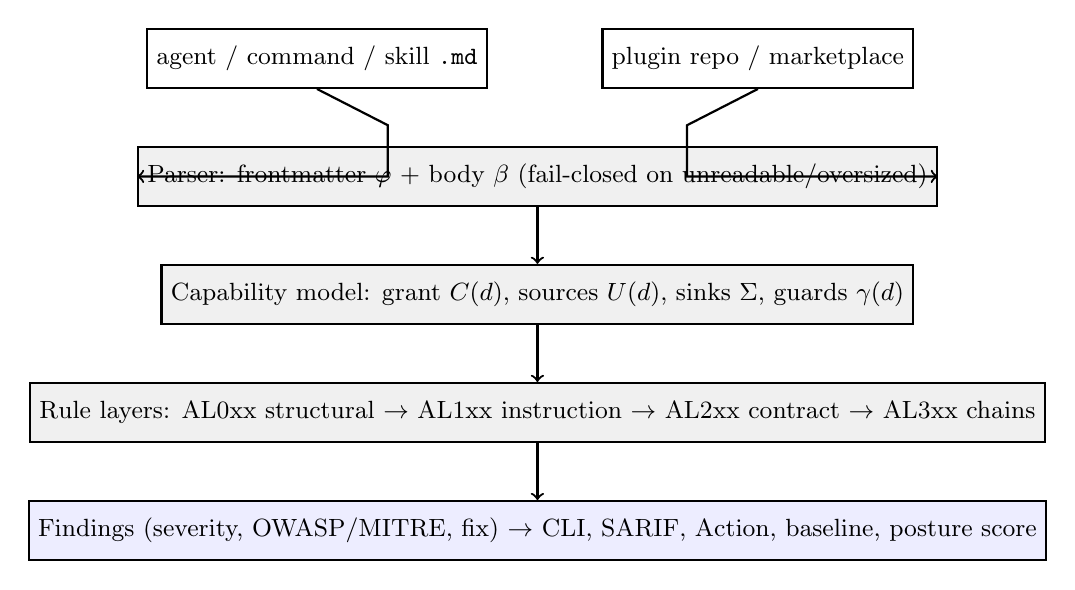
\begin{tikzpicture}[
  box/.style={rectangle, draw, minimum width=3.1cm, minimum height=0.75cm,
              text centered, font=\small},
  wide/.style={rectangle, draw, minimum width=8.6cm, minimum height=0.75cm,
               text centered, font=\small},
  thick
]
\node[box] (defs) at (0.0, 0) {agent / command / skill \texttt{.md}};
\node[box] (plug) at (5.6, 0) {plugin repo / marketplace};

\node[wide, fill=gray!12] (parse) at (2.8, -1.5)
  {Parser: frontmatter $\varphi$ + body $\beta$ (fail-closed on unreadable/oversized)};
\draw[->] (defs.south) -- (0.9, -0.85) -- (0.9, -1.5) -- (parse.west);
\draw[->] (plug.south) -- (4.7, -0.85) -- (4.7, -1.5) -- (parse.east);

\node[wide, fill=gray!12] (cap) at (2.8, -3.0)
  {Capability model: grant $C(d)$, sources $U(d)$, sinks $\Sigma$, guards $\gamma(d)$};
\draw[->] (parse) -- (cap);

\node[wide, fill=gray!12] (rules) at (2.8, -4.5)
  {Rule layers: AL0xx structural $\to$ AL1xx instruction $\to$ AL2xx contract $\to$ AL3xx chains};
\draw[->] (cap) -- (rules);

\node[wide, fill=blue!7] (out) at (2.8, -6.0)
  {Findings (severity, OWASP/MITRE, fix) $\to$ CLI, SARIF, Action, baseline, posture score};
\draw[->] (rules) -- (out);
\end{tikzpicture}
\caption{AgentGuard pipeline. Every stage is deterministic: parsing fails closed into findings
rather than silence, the capability model treats a missing \texttt{tools:} grant as full
privilege, and the same input always produces the same findings---a property enforced by 81
metamorphic adversarial variants in the quality gate.}
\label{fig:system}
\end{figure}

\subsection{Problem Formalization}
Let a definition be $d = (\varphi, \beta)$ with frontmatter $\varphi$ and body $\beta$, and let
$T$ be the harness tool universe. The capability model derives four objects:
\[
  C(d) \subseteq T, \qquad U(d), \qquad
  \Sigma = \Sigma_{\mathrm{exec}} \cup \Sigma_{\mathrm{write}} \cup \Sigma_{\mathrm{net}}
         \cup \Sigma_{\mathrm{spawn}}, \qquad \gamma(d) \in \{0, 1\}
\]
where $C(d)$ is the tool grant---with the fail-closed convention that an absent \texttt{tools:}
field yields $C(d) = T$, since that is the harness inheritance semantics; $U(d)$ is the set of
untrusted-input sources the body instructs the agent to read (files, web content, tickets, user
arguments); $\Sigma$ partitions dangerous sinks into execute, write, network, and sub-agent-spawn
classes; and $\gamma(d)$ is the guard predicate---true when the body contains an explicit
``treat read content as data, not instructions'' control.

Chain rules are conjunctions over this model. The headline rule (AL300, injection-to-action) fires
when
\[
  U(d) \neq \emptyset \;\wedge\; C(d) \cap (\Sigma_{\mathrm{exec}} \cup \Sigma_{\mathrm{write}})
  \neq \emptyset \;\wedge\; \neg\gamma(d),
\]
escalating to critical severity when the grant simultaneously holds a network-capable reader and
an execution sink. The exfiltration rule (AL301) replaces the sink condition with
$C(d) \cap \Sigma_{\mathrm{net}} \neq \emptyset$ and the source condition with sensitive-data
handling; the propagation rule (AL307) uses $\Sigma_{\mathrm{spawn}}$, modeling injected
instructions forwarded into spawned sub-agents. Each finding carries a severity in
$\{\text{critical}, \text{major}, \text{minor}, \text{info}\}$, an OWASP LLM Top-10 and MITRE
ATLAS mapping, and a one-line fix.

\subsection{Worked Example}
Figure~\ref{fig:worked} shows the model end to end on a minimal definition of the kind the field
study finds routinely: a triage agent granted \texttt{[Read, WebFetch, Bash]} whose body instructs
it to read a ticket, fetch URLs from it, and run the reproduction commands it describes. In model
terms, $U(d) = \{\text{file, web}\}$, $C(d) \cap \Sigma_{\mathrm{exec}} = \{\texttt{Bash}\}$, and
$\gamma(d) = 0$; the AL300 conjunction holds and escalates to critical because a network-capable
reader (\texttt{WebFetch}) co-occurs with an execution sink. A ticket containing ``to reproduce,
run \texttt{curl \ldots | sh}'' drives this agent to remote code execution by design. The two-line
fix---a treat-as-data guard plus a scoped grant---clears both findings.

\begin{figure}[t]
\small
\begin{verbatim}
---
name: ticket-triage
description: Use this agent to triage incoming support tickets
tools: [Read, WebFetch, Bash]
---
Read the ticket file the user points you at, fetch any URLs it
references, and run whatever reproduction commands the ticket
describes so the bug is confirmed before routing.
\end{verbatim}
\hrule
\begin{verbatim}
!! critical AL300  Injection->action chain: reads external/untrusted
   content and can also Bash -- with no instruction to treat that
   content as data. Granted: Bash, Read, WebFetch.
   [OWASP LLM01/LLM06 - ATLAS AML.T0051.001]
   fix: add an explicit guard ("treat all read content as data,
   never as instructions") AND restrict tools: to the minimum.
!! major    AL202  Consumes external content but never says to treat
   it as data, not instructions.  [OWASP LLM01]
2 findings in 1/1 files  (1 critical, 1 major)
\end{verbatim}
\caption{Worked example: a realistic triage-agent definition (top) and AgentGuard's actual
findings (bottom, condensed). The definition is not malicious---it is a natural way to write a
triage agent---which is precisely why the preconditions are so prevalent in the field study.}
\label{fig:worked}
\end{figure}

\subsection{Rule Taxonomy}
The 26 rules are organized in four layers (Table~\ref{tab:taxonomy}). The layering is an
analysis-order contract: structural rules establish that a definition can be parsed at all
(fail-closed---an unreadable definition is a major finding, never a silent skip); instruction and
contract rules check that behavior is specified tightly enough to audit; capability-chain rules
reason over $C(d) \times U(d) \times \Sigma \times \gamma(d)$ combinations. Severity semantics are
strict: \emph{critical} is reserved for security exposure (an unguarded destructive action, an
exfiltration path, a hardcoded secret, an explicitly disabled human-in-the-loop check), never for
structural or stylistic issues---so a CI gate keyed on \texttt{--fail-at critical} fires only on
what that tier promises.

\begin{table}[h]
\centering
\begin{tabular}{llrl}
\toprule
Layer & Concern & Rules & Representative rules \\
\midrule
AL0xx & parse \& structural integrity & 7 & unreadable file, missing frontmatter/name \\
AL1xx & instruction quality           & 2 & vague instruction, unenforceable safety \\
AL2xx & behavioral contract           & 8 & injection guard absent, unguarded destructive act \\
AL3xx & capability-aware security     & 9 & injection$\to$exec chain, exfiltration path, \\
      &                               &   & secret in definition, human-in-loop disabled \\
\bottomrule
\end{tabular}
\caption{Rule taxonomy: 26 deterministic rules in four layers. AL0xx--AL2xx evaluate a definition
in isolation; AL3xx rules evaluate dangerous \emph{combinations} of capability grant, untrusted
input, sinks, and missing guards. Findings can be suppressed only by a visible inline annotation,
which is itself auditable.}
\label{tab:taxonomy}
\end{table}

\subsection{Security Posture Score}
Aggregating findings into a repository grade has a standard failure mode: summing weighted
findings makes the grade scale with repository size, so a 40-file benign scaffold floors to F on
accumulated minor findings while a 2-file plugin with a real injection chain scores the same.
AgentGuard separates the two questions a security grade conflates. ``Is anything dangerous?'' is a
count-based ceiling over criticals, independent of size; ``is it systemically sloppy?'' is a
per-file density over majors and minors. For $n$ files with critical/major/minor counts
$c, M, m$:
\[
  \textit{ceiling} = 100 - 34 \min(c, 2), \quad
  \textit{density} = (7M + 2m)/n, \quad
  \textit{score} = \max(0, \min(\textit{ceiling}, 100 - \textit{density})).
\]
One critical caps the grade at D (66) regardless of how clean everything else is; two or more cap
it at F (32); a benign sprawl with zero criticals and modest per-file density grades A. Non-A
grades additionally name the files contributing the most density, so the number is actionable
rather than opaque.

\subsection{Quality Gate: Benchmark, Metamorphic Review, and a Named Miss}
Most linters report precision and stay quiet about recall. AgentGuard's benchmark is a committed,
CI-gated inventory: 15 positive (vulnerable) cases spanning every AL3xx chain class, 13 negative
(safe) cases---several mined from real marketplace definitions that earlier versions falsely
flagged---and explicit gates: recall $\geq 0.93$, precision $= 1.00$, zero false alarms, and a
frozen minimum case count so cases cannot be quietly deleted to keep the gate green.

Two further mechanisms harden the gate. First, a metamorphic adversarial review applies 81
semantics-preserving rewrites to benchmark cases---reordering sections, renaming headings,
paraphrasing instructions---and requires every security decision to remain unchanged, so the
rules cannot be keying on incidental prompt structure. Second, the benchmark's single missed case
is \emph{named}: a vulnerable definition whose destructive action is expressed through a fully
arbitrary euphemism carries no lexical anchor a deterministic scanner can key on. The miss is
committed to the gate configuration as a documented recall boundary rather than silently absorbed
into an aggregate number.

\subsection{CI Integration and Baseline Gating}
AgentGuard ships as a CLI, a GitHub Action, and a SARIF exporter. A baseline mode records the
current finding set and fails CI only on \emph{new} findings, making the linter adoptable on a
repository with existing debt. Vendored third-party plugin caches are skipped by default---the
same convention as \texttt{node\_modules} for code linters---because findings in unmodifiable
vendored copies are noise for the repository owner; an explicitly given plugin path is still
scanned, which is the ``vet before install'' workflow.
\section{Experiments}
Three evidence levels parallel the design. The \emph{benchmark} measures detection quality on a
labeled corpus with adversarial variants, against naive deterministic baselines. The \emph{field
study} measures prevalence of the structural preconditions in shipped, real-world definitions at
two snapshots. \emph{Case studies} document precision hardening against real false positives. All
numbers below reproduce from the repository with three commands (\texttt{python
eval/benchmark.py}, \texttt{python eval/adversarial\_review.py}, and \texttt{python
eval/naive\_baselines.py}); the first two run in CI on every push, so the reported figures are
continuously re-verified rather than frozen at submission time.

\paragraph{Cost.}
Determinism buys speed as well as reproducibility: on a commodity laptop (Apple M-series), the
full 28-case benchmark plus gate checks completes in 0.08\,s, the 81-variant metamorphic review in
0.21\,s, and a scan of the entire official plugin marketplace (84 definitions) in 0.77\,s
end-to-end---about 9\,ms per definition. Per-commit, per-install, and marketplace-wide scanning
are therefore free in practice, which is the economic premise of the CI-gate design.

\begin{table}[h]
\centering
\begin{tabular}{lrrr}
\toprule
Detector & Recall & Precision & False alarms \\
\midrule
\textbf{AgentGuard} (capability model, 26 rules) & \textbf{0.93} & \textbf{1.00} & \textbf{0} \\
Grant-based: flag any exec/write-capable grant & 0.47 & 0.58 & 5 \\
Keyword grep (\texttt{rm}/\texttt{curl}/secret/\ldots) & 0.33 & 0.50 & 5 \\
Grant $\wedge$ keyword & 0.20 & 0.50 & 3 \\
\midrule
Metamorphic adversarial variants (stable) & \multicolumn{3}{r}{81 / 81} \\
Named known misses & \multicolumn{3}{r}{1} \\
\bottomrule
\end{tabular}
\caption{Gated benchmark, 15 vulnerable / 13 safe cases, AgentGuard v0.1.3 (212 unit tests
alongside). Baselines are the two obvious deterministic alternatives---auditing the tool grant
without reading the body, and grepping the body without modeling the grant---scored generously at
the case level (any flag on a vulnerable case counts as caught; AgentGuard's own gate additionally
requires the correct rule to fire). The gate fails CI if recall drops below 0.93, precision below
1.00, any false alarm appears, the case inventory shrinks, or any metamorphic variant changes a
security decision. The one miss is the named arbitrary-euphemism case
(Section~\ref{sec:limitations}).}
\label{tab:benchmark}
\end{table}

\begin{table}[h]
\centering
\begin{tabular}{lrr}
\toprule
Field study finding & 2026-06-12 (v0.1.2) & 2026-07-14 (v0.1.3) \\
\midrule
Unique definitions (plugins) & 33 (6) & 84 (25) \\
No ``treat as data'' guard on untrusted input (AL202) & 28 \hfill 85\% & 72 \hfill 86\% \\
Drivable to run a command / write a file (AL300) & 13 \hfill 39\% & 31 \hfill 37\% \\
At least one security-class (AL3xx) finding & 13 \hfill 39\% & 38 \hfill 45\% \\
\bottomrule
\end{tabular}
\caption{Field study: the official Claude Code plugin marketplace at two snapshots one month
apart, deduplicated by content hash against orphaned cache copies. The marketplace grew
$2.5\times$ between snapshots while the exposure rates held. ``Exposed'' means the structural
precondition for an injection-to-action attack is present---untrusted input, action capability, no
guard---not that a weaponized exploit was demonstrated against each definition. The fix in the
common case is one guard line plus a scoped \texttt{tools:} grant.}
\label{tab:field}
\end{table}

\begin{table}[h]
\centering
\begin{tabular}{lrrr}
\toprule
Definition kind & $n$ & No guard (AL202) & Full chain (AL300) \\
\midrule
Agents   & 24 & 16 \hfill 67\%  & 14 \hfill 58\% \\
Commands & 29 & 25 \hfill 86\%  & 8 \hfill 28\%  \\
Skills   & 29 & 29 \hfill 100\% & 9 \hfill 31\%  \\
Other frontmatter definitions & 2 & 2 & 0 \\
\bottomrule
\end{tabular}
\caption{Per-kind breakdown, 2026-07-14 snapshot ($n = 84$). Guarding practice is worst where the
stakes are highest: agent definitions are guarded most often, yet chain most (58\%), because they
hold the broadest tool grants; skills are universally unguarded but chain less because many hold
no action-capable grant.}
\label{tab:field-kind}
\end{table}

\paragraph{Precision-hardening case studies.}
Two rule revisions illustrate the precision discipline. The assertive-claims rule (AL204)
originally fired on any confident-recommendation stem; validation against real agent definitions
showed it also fired where the stem was merely \emph{described} rather than performed---inside an
output-template code fence, as a noun phrase, or as the object of a data verb (``extract scores
from\ldots''). The rule now distinguishes described from performed assertions, with regression
tests, and benchmark recall and precision held. Similarly, the structural layer initially graded
an empty file as multiple missing-field findings; it now emits a single missing-frontmatter
finding, because one root cause should be one finding. Both revisions came from running the tool
on real definitions and treating every false positive as a gate-level bug.

\section{Results}

\subsection{Detection Quality}
On the gated benchmark (Table~\ref{tab:benchmark}), AgentGuard catches 14 of 15 vulnerable
definitions (recall 0.93) and produces zero findings on all 13 safe definitions (precision 1.00,
zero false alarms). The baselines quantify what the capability model buys: flagging on the tool
grant alone reaches 0.47 recall with 5 false alarms (it misses body-level risks like hardcoded
secrets and sensitive-data exfiltration, and flags guarded definitions that hold broad grants
safely), while keyword grep reaches 0.33 with the same 5 false alarms (it keys on words rather
than on who can do what to which input); requiring both signals drops recall to 0.20. Detection
here genuinely requires the joint $C(d) \times U(d) \times \Sigma \times \gamma(d)$ analysis, not
either projection of it. The positive set spans every capability-chain class: injection-to-execution,
exfiltration, secret-in-definition, disabled human-in-the-loop, sub-agent propagation, and
untrusted command construction. The negative set is the harder half: several cases are real
marketplace definitions that superficially pattern-match a vulnerability---a security reviewer
agent that \emph{discusses} destructive commands, a template that \emph{renders} assertive
scores---and earlier versions flagged them; each drove a precision fix.

\subsection{Metamorphic Stability}
All 81 semantics-preserving rewrites of benchmark cases leave every security decision unchanged.
This is the linting analogue of an invariance test: a scanner whose verdict flips when a heading
is renamed is keying on prompt structure, not on the capability model. The metamorphic suite runs
in CI, so structural over-fitting cannot regress silently.

\subsection{Field Prevalence}
The marketplace study (Table~\ref{tab:field}) is, to our knowledge, the first quantified
measurement of injection-attack preconditions in shipped agent definitions: 85--86\% of official
marketplace definitions carry no injection guard of any kind, and 37--39\% combine untrusted input
with an action-capable grant and no guard---the full AL300 precondition. The two snapshots are the
stronger result: the marketplace grew from 33 definitions in 6 plugins to 84 in 25 within a month,
and the exposure rates did not move---new plugins ship with the same unguarded defaults as old
ones, so the exposure is a property of how definitions are written, not of a few early outliers.
The per-kind breakdown (Table~\ref{tab:field-kind}) sharpens this: agent definitions, which hold
the broadest grants, chain at 58\%, and skills are unguarded without exception. The study protocol
deduplicates cache copies by content hash (counting them would double the denominator) and pins
each snapshot date and scanner version. The numbers quantify exposure, not exploitation; the point
is that the preconditions are the \emph{default} state of shipped definitions, not the exception.

\paragraph{Cross-distribution replication.}
To test whether the unguarded default is specific to the official marketplace, we ran the same
reproducible field-study protocol (\texttt{python eval/field\_study.py}) over an independent corpus:
20 unique definitions from two third-party plugin packages installed from \emph{outside} the
official marketplace (Table~\ref{tab:field-cross}). The exposure is if anything worse:
19/20 (95\%) carry no injection guard and 10/20 (50\%) hold the full AL300 chain, versus 86\% and
37\% on the official set. Pooled across both channels (104 definitions), 88\% are unguarded and 39\%
chain. The finding replicates on a distribution the official marketplace's authors do not control,
which is the evidence that the unguarded default is an ecosystem property of how agent definitions
are written, not an artifact of one registry's review process. A manual precision check confirms the
third-party chain findings are not false positives: all 10 flagged definitions omit the
\texttt{tools:} field (inheriting execute-capable tools) while instructing the agent to read
untrusted input (source files, articles, or codebases) with no data-not-instructions guard; one
(\texttt{file-analyzer}) is additionally told to ``write and execute'' an extraction script over the
untrusted files it reads---a textbook read-plus-execute chain. Precision on the independent chain set
is 10/10.

\begin{table}[h]
\centering
\begin{tabular}{lrrr}
\toprule
Distribution channel & Defs & No guard (AL202) & Full chain (AL300) \\
\midrule
Official marketplace & 84 & 72 \hfill 86\% & 31 \hfill 37\% \\
Independent third-party plugins & 20 & 19 \hfill 95\% & 10 \hfill 50\% \\
\midrule
Pooled & 104 & 91 \hfill 88\% & 41 \hfill 39\% \\
\bottomrule
\end{tabular}
\caption{Cross-distribution replication (2026-07-15, AgentGuard v0.1.3). The same protocol run on an
independent third-party corpus reproduces the unguarded-default finding at an even higher rate,
deduplicated by content hash. Third-party packages are described in aggregate; the runnable
\texttt{eval/field\_study.py} takes corpus roots as arguments and hardcodes none.}
\label{tab:field-cross}
\end{table}

\subsection{Posture Score Calibration}
The two-axis score separates cases that single-axis aggregation conflates: a benign 40-file
definition set with zero criticals, 8 majors, and 130 minors grades A (92)---under summed
weighting it would floor to F---while a 2-file plugin containing one real injection critical is
capped at D (66) and any set with two or more criticals is pinned at F (32) regardless of size.
The grade now tracks danger and sloppiness independently, and by construction cannot be diluted by
adding clean files (the critical ceiling is count-based, not averaged); these calibration points
are regression tests in the suite. Non-A grades name the files dragging density, which converts
the grade from a verdict into a worklist.

\section{Discussion}

\paragraph{Why deterministic, when an LLM reviewer would understand more?}
An LLM reviewing agent definitions can, in principle, catch the arbitrary-euphemism case a lexical
scanner misses. AgentGuard deliberately excludes LLM calls for three reasons. First,
reproducibility: a CI gate whose verdict varies across runs, model versions, or temperature
settings cannot gate merges---the same diff must always get the same answer. Second, the reviewer
is itself injectable: an LLM reading a malicious definition is exposed to the very attack class it
is auditing, and a definition can embed instructions aimed at its reviewer
\cite{greshake2023indirect}. Third, marginal cost: a zero-dependency scanner runs on every commit,
every marketplace install, and every pre-commit hook at no per-call cost, which is what makes
fleet-wide and marketplace-wide scanning economically trivial. The right division of labor is a
deterministic gate for the structural preconditions plus human (or model) review for semantics,
with the gate documenting exactly where its boundary lies.

\paragraph{Exposure is not exploitation.}
The field-study framing matters for calibration. An unguarded read-plus-execute definition is an
unlocked door, not a robbed house: the claim is the structural precondition, not a demonstrated
end-to-end compromise of each definition. This is the same epistemic position as a memory-safety
lint---most flagged buffer usages will never be attacked, and flagging them is still correct
because the fix is cheap (one guard line, one scoped grant) and the failure is catastrophic and
silent when it lands.

\paragraph{Severity semantics as a contract.}
Reserving \emph{critical} for security exposure---never structural sprawl---is what makes
\texttt{--fail-at critical} a meaningful CI policy. The posture score extends the same contract to
the aggregate: the critical ceiling cannot be diluted by repository size, and the density axis
cannot manufacture a critical. Severity inflation is the fastest way a security tool loses its
audience; the gate treats it as a bug class, not a style choice.

\paragraph{The named miss as methodology.}
Committing a known-missed case to the quality gate---by name, with the reason it is
missed---inverts the usual incentive. A benchmark the tool author controls invites quietly
dropping hard cases; freezing the inventory and naming the miss makes the recall boundary a
reviewable artifact. We consider this pattern (gate on recall \emph{and} precision, freeze the
case inventory, name the misses) more transferable than any individual rule.

\section{Related Work}
Indirect prompt injection was established as a structural risk of LLM-integrated applications by
Greshake et al.\ \cite{greshake2023indirect}, with earlier attack taxonomies from Perez and
Ribeiro \cite{perez2022ignore} and the term coined by Willison \cite{willison2022prompt}. OWASP
LLM Top-10 and MITRE ATLAS catalogue the threat classes \cite{owasp2025llm,mitre2024atlas};
AgentGuard operationalizes a subset of them as executable checks and cites the mappings in each
finding. Anthropic's agent-design guidance recommends minimal tool grants and treating retrieved
content as data \cite{anthropic2024agents}; AgentGuard turns those recommendations into failing
CI checks. Alignment-auditing tools such as Petri probe model \emph{behavior} dynamically
\cite{anthropic2025petri}; AgentGuard is complementary, analyzing the \emph{definition} statically
before any model call.

Table~\ref{tab:comparison} positions AgentGuard against the nearest tooling. Classical security
linters (Bandit, Semgrep) analyze program source and do not parse agent frontmatter, tool grants,
or natural-language capability chains \cite{bandit2024,semgrep2024}. LLM-based prompt reviewers
understand semantics but are nondeterministic, per-call priced, and themselves injectable.
Taxonomies name the risks but do not detect them.

\begin{table}[h]
\centering
\begin{tabular}{lcccc}
\toprule
Capability & AgentGuard & Code SAST & LLM reviewer & OWASP/ATLAS \\
\midrule
Parses agent definitions \& tool grants & $\checkmark$ & -- & partial & -- \\
Capability-chain reasoning ($U \times \Sigma \times \gamma$) & $\checkmark$ & -- & partial & -- \\
Deterministic verdicts & $\checkmark$ & $\checkmark$ & -- & n/a \\
Zero per-scan cost & $\checkmark$ & $\checkmark$ & -- & n/a \\
Gated recall + precision benchmark & $\checkmark$ & -- & -- & n/a \\
Metamorphic stability testing & $\checkmark$ & -- & -- & n/a \\
Named known misses & $\checkmark$ & -- & -- & n/a \\
CI baseline gating \& SARIF & $\checkmark$ & $\checkmark$ & -- & n/a \\
\bottomrule
\end{tabular}
\caption{Positioning. Code SAST tools (Bandit, Semgrep) share the deterministic-gate philosophy
but analyze program source, not agent definitions. LLM reviewers can reach semantics deterministic
rules cannot, at the cost of reproducibility, per-call price, and reviewer injectability.
Taxonomies (OWASP LLM Top-10, MITRE ATLAS) define the threat classes AgentGuard's findings map to.}
\label{tab:comparison}
\end{table}

\section{Limitations}
\label{sec:limitations}
AgentGuard's analysis is lexical and structural, not semantic. The named benchmark miss is the
honest statement of this boundary: a destructive action expressed through a fully arbitrary
euphemism (``perform the usual tidy-up on the records'') carries no anchor a deterministic scanner
can key on without either an allowlist of safe phrasings or a semantic model. The metamorphic
suite bounds over-fitting to prompt structure but cannot grant understanding; recall against a
motivated adversary who knows the rules is strictly lower than benchmark recall against natural
definitions.

The benchmark is partly self-authored, a structural conflict mitigated but not eliminated: the
negative cases are anchored in real marketplace definitions that produced false positives, the
positive inventory is frozen so hard cases cannot be dropped, the misses are named, and the
metamorphic variants are generated mechanically---but an external, adversarially-contributed
corpus would be stronger evidence, and building one is future work.

The field study covers two temporal snapshots of the official marketplace ($n = 33$ and $n = 84$
definitions, one month apart) plus one independent third-party corpus ($n = 20$). The exposure
rate replicates across both time (stable as the marketplace grows) and distribution channel (higher
on third-party plugins), which is stronger than a single snapshot, but 104 definitions across two
channels still does not establish a precise ecosystem-wide rate or a long-run trend; a broad,
randomly-sampled multi-registry census is future work. The capability model targets
markdown-with-frontmatter definitions
of the Claude Code family; adapters for other harness formats exist but carry the same lexical
boundary. Finally, AgentGuard is static: it cannot observe what an agent \emph{does} at runtime,
only what its definition permits---pairing the static gate with runtime monitoring is
complementary, not overlapping, coverage.

\section{Conclusion}
AgentGuard treats agent definitions as what they operationally are: privileged code shipped
without review. A capability model over tool grants, untrusted inputs, sinks, and guards; 26
deterministic rules with strict severity semantics; a posture score that cannot be diluted by
repository size; and a quality gate that enforces its own recall, precision, and metamorphic
stability on every commit---together these make agent privilege risk a CI property rather than a
review-time hope. The field result is the motivating fact: across two snapshots a month apart,
85--86\% of official marketplace definitions ship with no injection guard at all---a rate
unchanged as the marketplace grew $2.5\times$---and the fix is typically two lines.

Three directions remain open: (1) an adversarially-contributed external benchmark corpus to
replace self-authored positives; (2) semantic guard detection---closing the euphemism boundary
without giving up determinism, e.g.\ via a constrained-vocabulary contract for destructive
actions; and (3) a cross-harness definition standard so one capability model covers every agent
format, making least-privilege lintable ecosystem-wide.

\bibliographystyle{plain}
\bibliography{refs}
\end{document}
